\documentclass{article}
%基于北京航空航天大学仪器科学与光电工程学院实验报告及课程报告排版得来,类似于毕业论文排版格式
%后续将更新毕业论文排版格式
\usepackage{graphicx,float}%使用图的宏包,使用图的浮动体宏包,引入参数H使图像紧跟当前文字
\usepackage{caption} %使用图表标题的宏包
\usepackage[colorlinks=true,pdfstartview=FitH,%
linkcolor=black,anchorcolor=violet,citecolor=magenta]{hyperref}%加载hyperref宏包,使用超链接
\usepackage{setspace}%用于设置行间距列间距等命令的宏包
\usepackage{array}%设置列表高度宽度的宏包
\usepackage{zhnumber}%使用中文数字编号的宏包
\usepackage{titlesec,titletoc}%使用标题自定义形式的宏包和使用目录自定义形式的宏包
\usepackage{siunitx}%物理学单位宏包
\usepackage{tabularx}%让表格宽度等于页面宽度
\usepackage{makecell}%单个表格单元调整的宏包
\usepackage{subfigure} %%使用子图的宏包
\usepackage{dirtree}
\usepackage[backend=biber,%nature,%%加载biblatex宏包,使用参考文献
gbnamefmt=quanpin,%将文献作者姓氏区分大小写
bibstyle=gb7714-2005,%加载参考文献样式表
maxbibnames=3,
%nature,%%加载biblatex宏包,使用参考文献
citestyle=gb7714-2005,%加载引注样式
%backref=false,%不显示引用文献的页码
gblocal=gb7714-2005,%使中英文献各自输入中英文的“和”与“等”
url=false,%注意,report类型文档类下,url和报告时间是必须的
doi=false,%不显示网址和doi
gbpunctin=false,%不显示文献中的//析出符号
gbmedium=false,%不显示OL符号
mergedate=none
]{biblatex}%标注(引用)样式citestyle,著录样式bibstyle都采用gb7714-2015样式
% \usepackage{pgfplots}%类似tikz的一个画图库,主要画统计图
\usepackage{../customStyle}
\addbibresource[location=local]{bibliography.bib}
\graphicspath{{./fig}}

\fancyhf{} 
% 页眉页脚设置
\lhead{陈博非}
\chead{实验室服务器使用说明}
\rhead{\today}
\cfoot{\thepage}
\rfoot{}
\lfoot{}

% 表格行间距调整为1.5
\renewcommand{\arraystretch}{1.5}

\begin{document}
% 加入页眉页脚
\thispagestyle{fancy}
\section{服务器基本情况}
实验室现有两台服务器,其基本信息如表\ref{tab:server}所示:
\begin{table}[H]
  \centering
  \caption{服务器基本信息}
    \begin{tabular}{ccccccc}
      \toprule
       序号&IP地址& 端口 & 系统版本 & CPU & 内存& 显存 \\
      \hline
      \#1& 10.131.150.189& 20022& Ubuntu18.04&  Intel(R) Xeon(R) Silver 4215R CPU& 192GB& 3090 $\times$8 \\
      \#2&10.131.150.189 &20023&Ubuntu20.04& Intel Core(TM) i9-9900X CPU & 64GB & 2080Ti $\times$4\\
       \bottomrule
  \end{tabular}
  \label{tab:server}
\end{table}
两台服务器当前都位于学院路简易房内,由学校开放校园网网关接入校园网中,可直接使用SSH连接,远程使用。同理,实验室内网也接入校园网,亦可以通过内网直接连接服务器。
\section{你的账号}
基本信息如表\ref{tab:user}所示。
\begin{table}[H]
  \centering
  \caption{账号信息}
  \resizebox{\linewidth}{!}{
  \begin{tabular}{cccc}
      \toprule
       用户名& 密码 & 权限 & 服务器 \\
      \hline
       \code{a804\_qkf} & \code{123456} & 普通用户& \#2\\
       \bottomrule
  \end{tabular}}
  \label{tab:user}
\end{table}
\section{快速使用说明}
\subsection{远程连接}
在Windows本地端连接至服务器,可参考以下步骤:
\begin{enumerate}
  \item 打开命令行cmd,输入\code{ssh -p 20023 a804\_qkf@10.131.150.189}。
  \item 输入密码,即可连接至服务器
\end{enumerate}
如使用\code{pycharm}、\code{vscode}等IDE,可查询相关教程,只要此处能登录,教程内的方法即可使用,此处不再多言,登录后的界面如图\ref{fig:成功登录界面}所示:
\begin{figure}[H]
  \centering
  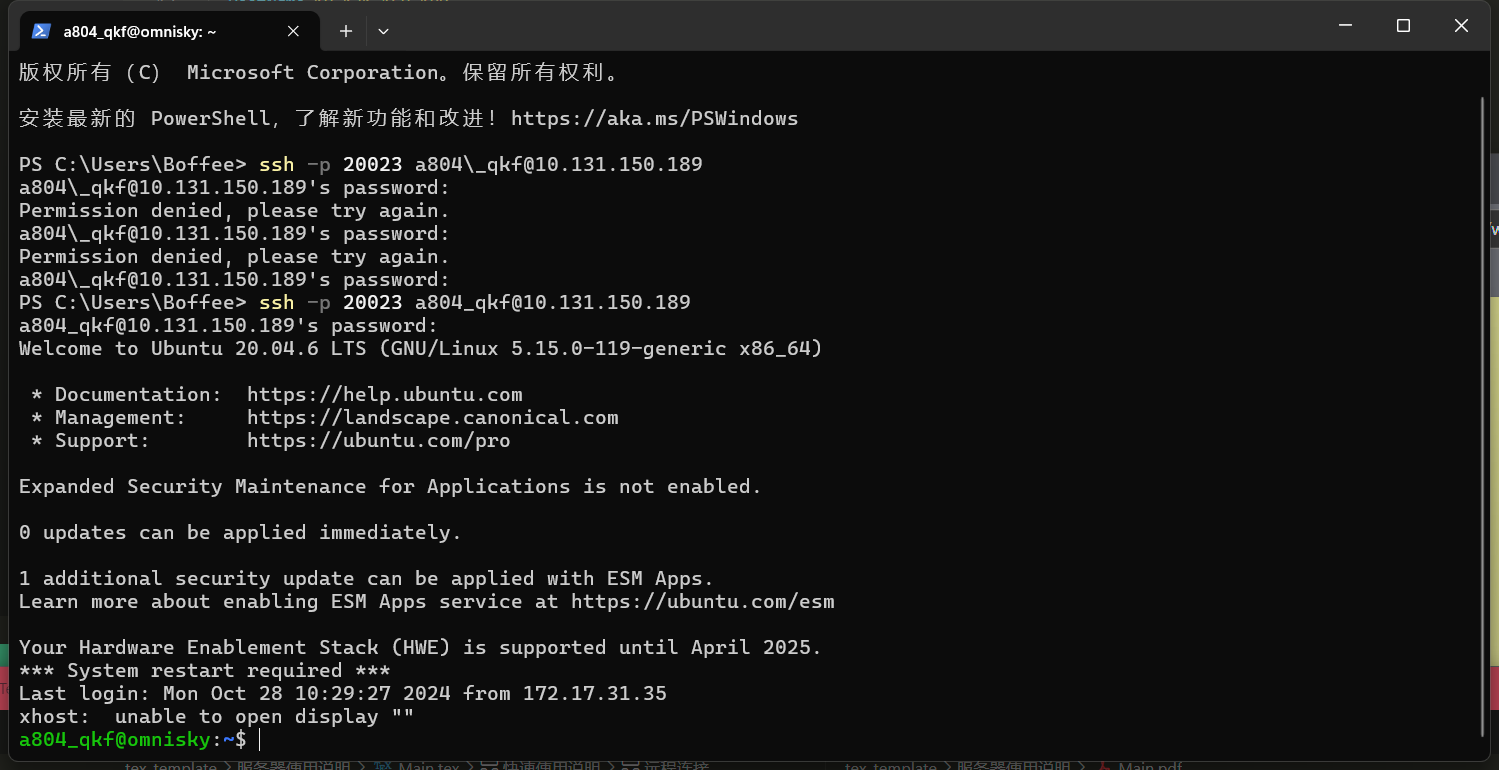
\includegraphics[width=0.8\textwidth]{成功登录界面.png}
  \caption{命令行登录成功界面}
  \label{fig:成功登录界面}
\end{figure}
\subsection{Linux系统快速上手}
使用Linux系统是程序员的基本技能,Linux系统的一大特点是只能通过命令行与操作系统交互。建议熟悉掌握以下常用命令:
  % \resizebox{\linewidth}{!}
  % {
  \begin{longtable}{cc}
    \caption{Linux常用命令}
    \label{tab:Linux常用命令}\\
    \toprule
    命令& 作用\\
    \hline
    \code{cd} & 前往指定目录,如\code{cd /home/a804\_qkf}\\
    \code{ls} & 列出当前目录下的文件,更常用的是它的快捷键\code{ll},可列出详细信息\\
    \code{mv} & 移动文件至另一目录、重命名\\
    \code{cp} & 复制文件\\
    \code{rm} & \makecell[c]{删除文件,加入参数\code{-r }可递归地删除文件夹\\ \textbr{注意!删除一定慎重,服务器上没有启用回收站功能,删除后文件将不可找回}}\\
    \code{mkdir} & 创建文件夹\\
    \code{touch} & 创建文件\\
    \code{|} & 管道运算符,搭配\code{grep}、\code{xargs}、\code{sed}等命令食用更佳\\
    \code{cat} & 查看文件内容\\
    \code{vim} & 编辑文件,\code{vimtutor}可查看教程\\
    \code{top} & 查看系统资源使用情况\\
    \code{ps} & 查看进程\\
    \code{kill} & 杀死进程\\
    \code{scp} & \makecell[c]{从服务器下载文件至本地,亦可上传文件至服务器\\ 如\code{scp -P 20023 /home/a804\_qkf/test.txt  a804\_qkf@10.131.150.189}}\\
    \code{ln} & 快速创建软链接\\
    \code{find} & 查找文件\\
    \bottomrule
   
  \end{longtable}
  % }
  
\subsection{注意事项}
\begin{enumerate}
  \item 网上的教程多数没有考虑自定义端口\code{20023},请务必注意。
  \item 可以配置\code{ssh}的\code{config}文件,使得SSH连接可用快捷键、支持直连(不需要重复输入密码),详情请自行google。
  \item 建议登录系统后立即使用命令\code{passwd}修改密码。
\end{enumerate}
\section{数据集}
现有的陨石坑导航流程可以分为两类,一种是利用检测或分割网络提取陨石坑、识别陨石坑并解算位姿(称为传统模式识别的方法);另一种方式是利用检测或分割网络提取陨石坑,然后求解陨石坑的子图与地图的特征点匹配关系,进而解算位姿(称为基于场景识别的方法)。这两种方式都需要检测陨石坑作为为前提,因此练手项目可以就是检测陨石坑。
\subsection{遥感数据}
现有数据集分为两类,一类是月球全球的数据集,另一类是局部区域的数据集,可以下载的位置位于\href{https://astrogeology.usgs.gov/search?pmi-target=moon}{NASA LROC项目官网}里面包括了各类探测项目的各种遥感地图,包括DEM和遥感图像、红外图像等。服务器上已经下载了部分遥感地图可以直接使用,见于:
\subsubsection{嫦娥五号遥感地图}
数据集路径:
\code{/disk527/DataDisk/a804\_cbf/datasets/lunar\_crater/chang\_e}
内有文件:
\dirtree{%
.1 /disk527/DataDisk/a804\_cbf/datasets/lunar\_crater/chang\_e.
.2 Liu\_chang\_e\_5\_annotation.txt.
.2 M1173414625\_DEM\_clip.tif.
.2 M1173414625\_DEM.tif.
.2 M1348581418LE\_DEM.tif.
.2 NAC\_ROI\_CHANGE5\_LOA\_E432N3091.IMG.
.2 NAC\_ROI\_CHANGE5\_LOA\_E432N\_clip.tif.
.2 Qian\_chang\_e\_5\_annotation.csv.
.2 \textbr{README.md}.
}
其中的\code{README.md}文件内有详细介绍各个子文件的具体的位置、投影方式和分辨率,带有后缀“clip”的是从不带后缀的原图中裁剪出来的。
\subsubsection{Kayuga遥感地图}
\code{/disk527/DataDisk/a804\_cbf/datasets/lunar\_crater/global}
月球全球的数据集,投影方式等细节见于README.md文件。
\subsubsection{月球南极遥感地图}
\code{/disk527/DataDisk/a804\_cbf/datasets/lunar\_crater/pole}
说明:各个\code{.LBL}文件里面含有说明信息,包括投影方式和分辨率、经纬度等信息。
\subsection{有标注的数据集}
以上提到的数据集都不是带标注的,
\subsubsection{WAC数据集}
这个数据集来自于文献\cite{yangCraterDANetConvolutionalNeural2022},它的数据存储格式是:图像名.png、图像名.txt;其中标注框位于\textbr{图像名.txt}文件中。采用的是\code{x,y,w,h}格式。该数据集位于:
\code{/disk527/sdb1/a804\_cbf/datasets/CraterDANet}。其中还有一个\code{visualize.py}文件,可以可视化显示某张图像的标注框(需要在你自己的目录下使用,在我的目录下你没有执行权限)。
\subsubsection{嫦娥五号数据集}
\label{sec:嫦娥五号数据集}
这个数据集的标注文件来自于文献\cite{liuIdentificationLunarCraters2024},截取了嫦娥五号着陆点附近的部分图像制作而来,其中有标注的图像位于\code{test}和\code{train}目录下。文件夹下的\code{.txt}文件是标注陨石坑集合,每行从左至右分别是北纬、东经和直径(m)。该数据集下有\code{100}、\code{300}、\code{500}、\code{1000}四个分辨率的数据集,代表的是裁剪原图的尺寸并压缩至256$\times$256分辨率。
\section{当前任务}
当前最急需的任务是构建一个高精度的着陆地区陨石坑目录,例如嫦娥五号着陆地区,即针对第\ref{sec:嫦娥五号数据集}条中的无标注数据集,利用现有的陨石坑目录和标注数据集,训练陨石坑标注网络,完成对嫦娥五号着陆点附近小型陨石坑的标注。\par
因此,可以从陨石坑检测方面上手,先训练一个能够从图像中提取陨石坑的网络,可以尝试多个不同的模型,比较它们的结果。再选一个最好的模型,去无标注图像上检测陨石坑,生成目录。
\subsection{现有检测模型}
现有陨石坑检测模式大多基于计算机视觉的目标检测领域或者图像分割领域。如以下多篇文献:
\begin{table}[H]
  \centering
    \begin{tabular}{c|c}
      \toprule
      文献& 说明\\
      \hline
      pyCDA\cite{cohenCraterDetectionConvolutional2016}&使用DEM数据作CNN的检测网络,详见于\href{https://github.com/AlliedToasters/PyCDA?tab=readme-ov-file}{项目地址}\\
      DeepMoon\cite{leeAutomatedCraterDetection2019} & 基于Unet的,使用DEM数据作的分割网络,详写于\href{https://github.com/silburt/DeepMoon}{项目地址}\\
      \bottomrule
    \end{tabular}
\end{table}
除了这些模型以外,还可以选用更普遍意义上的检测网络,如Faster R-CNN、YOLOX、YOLOv5、SSD、DETR等,都可以用来做陨石坑检测尝试。
\newpage
\printbibliography[heading=bibliography,title=参考文献]
\end{document}
